\chapter{Lahanai Dolma}
\label{ch:lahanai_dolma}
\index{meal}
\index{meat}
\index{tomato}
\index{cabbage}

\marginnote{
    \textbf{Makes 6-8 servings} \\
    Prep time: 30-40 minutes \\
    Cook time: 45 minutes \\
    \vspace*{\baselineskip}
    
    1/2 savoy cabbage \\
    1 lb of ground beef \\
    1/4 cup + 1 tbsp rice, Calrose \\
    1 medium onion, chopped \\
    1/2 tsp salt \\
    1/2 tsp pepper \\
    3/4 cup + 1/4 - 1/3 cup Passata, Unico (low sodium)
}

\begin{figure}
  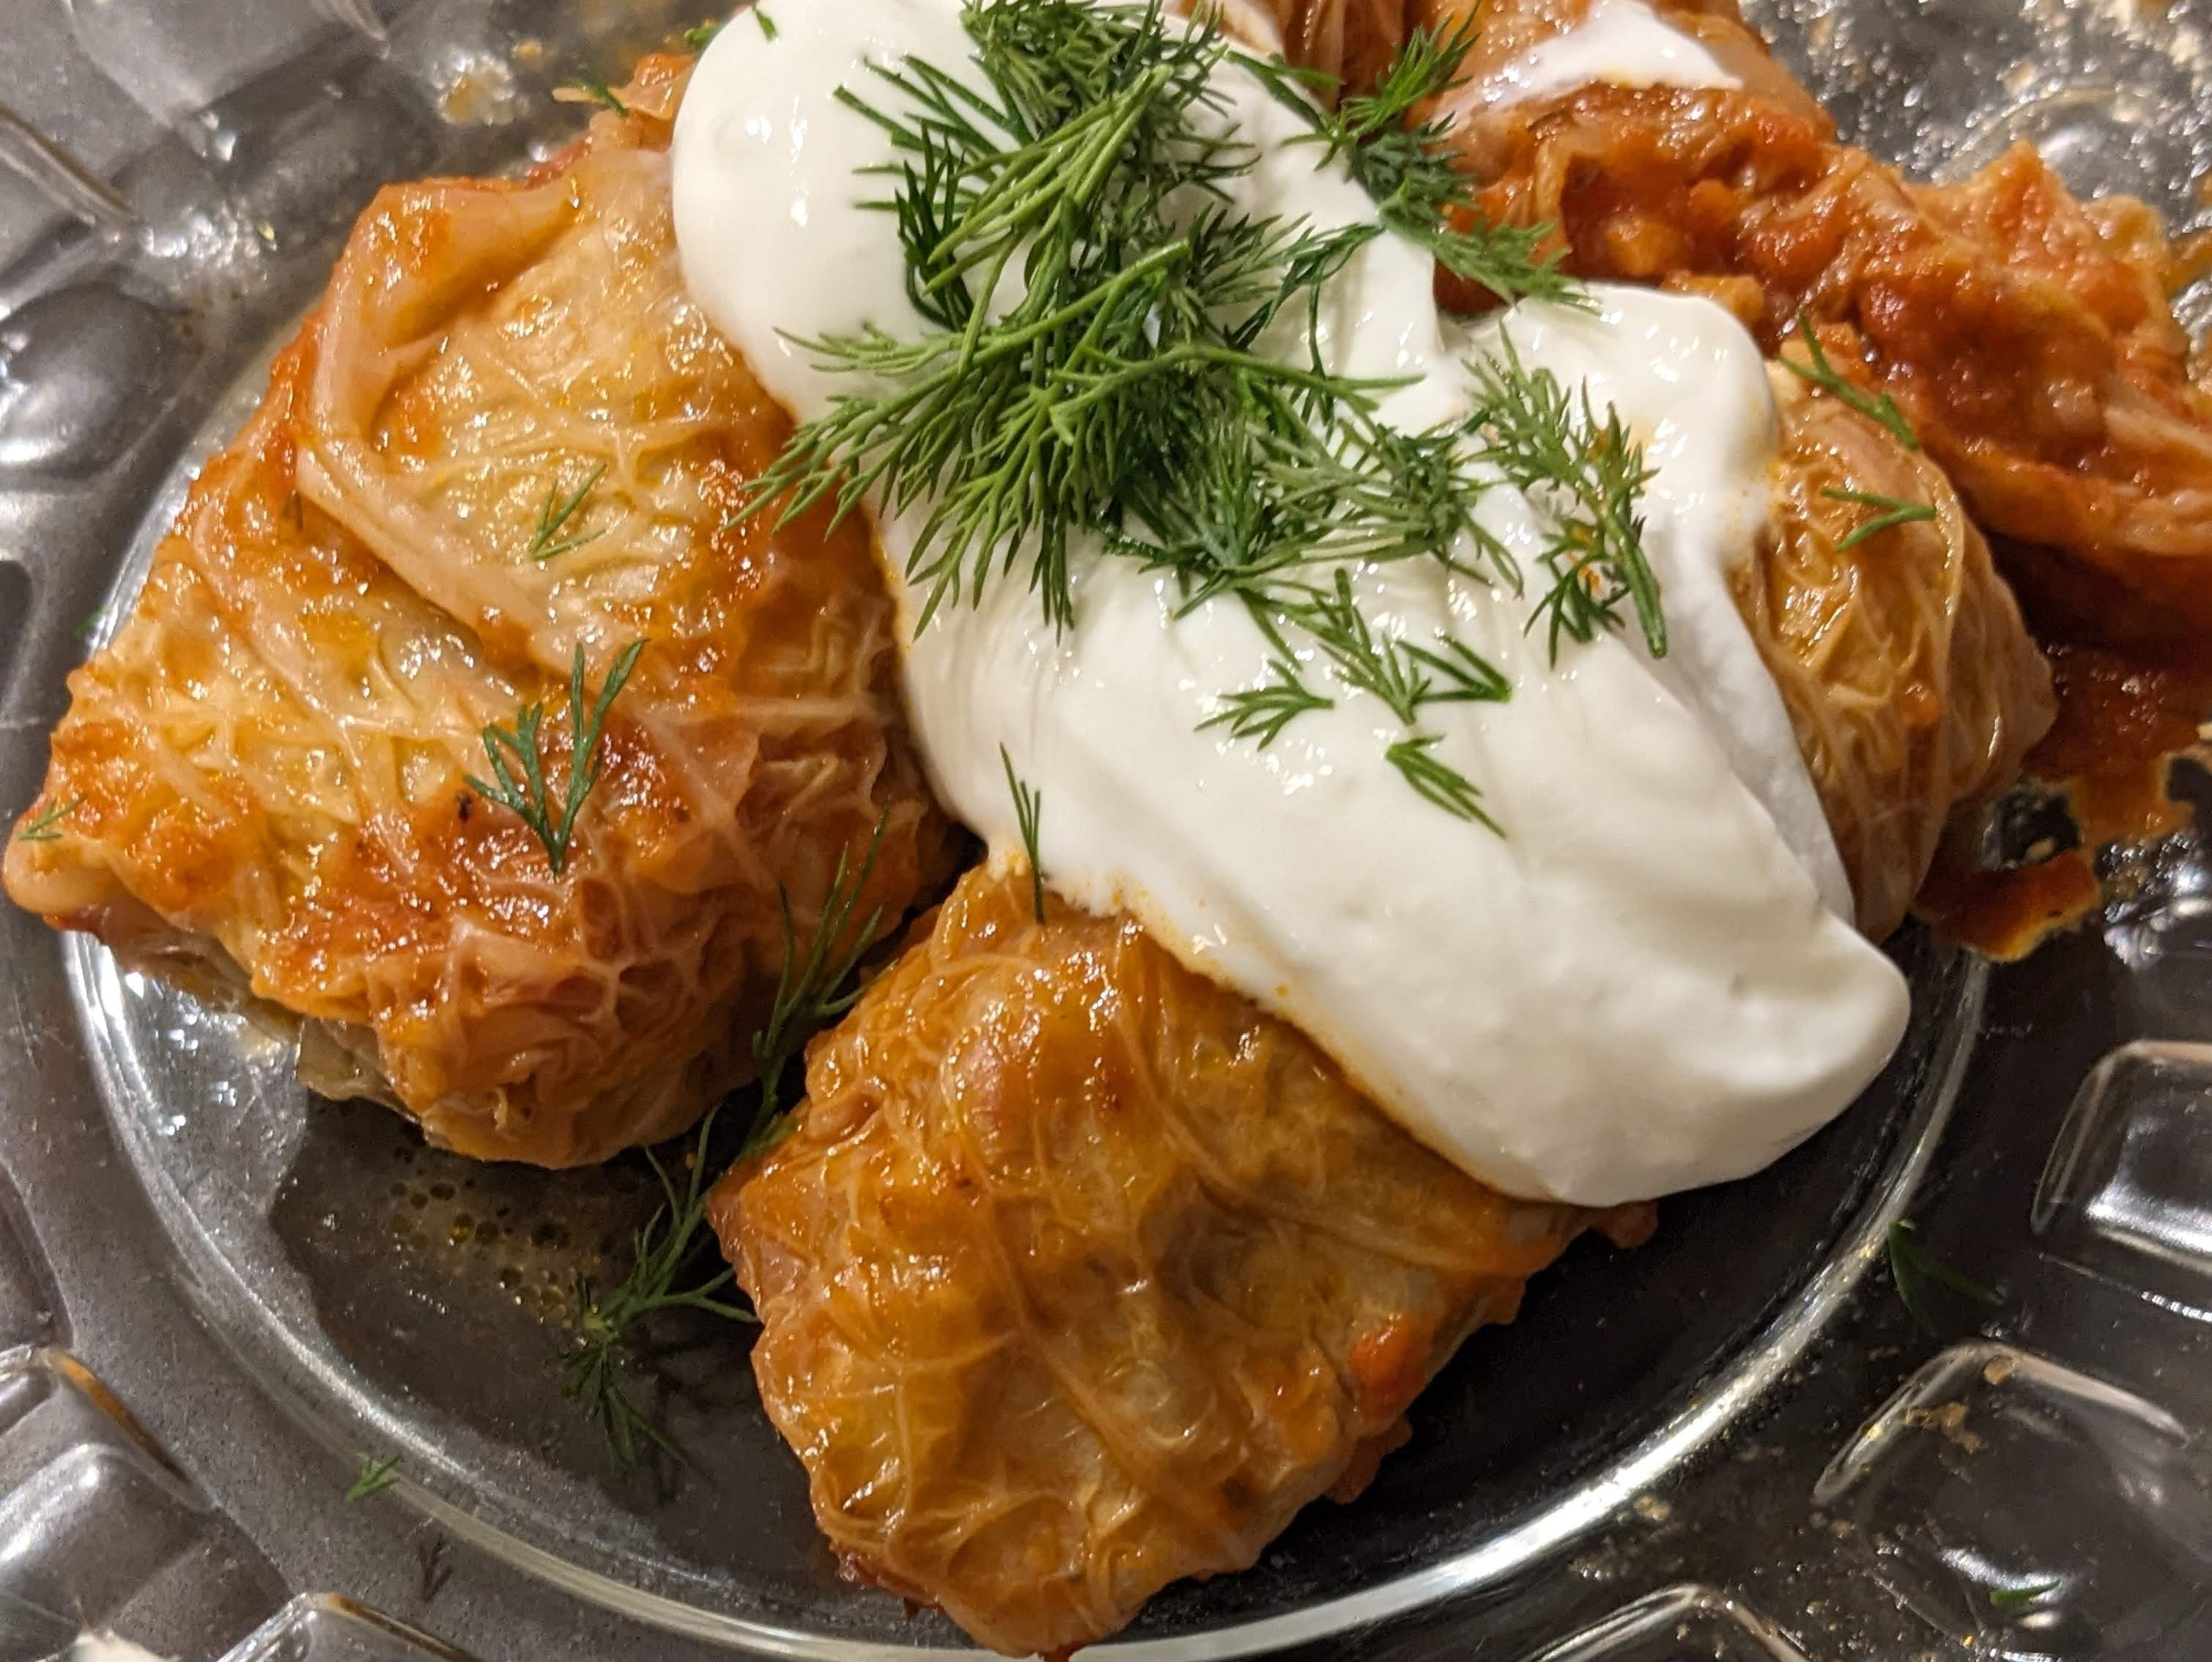
\includegraphics[width=60mm]{dermardiros/images/PXL_20240128_010747331.PORTRAIT.ORIGINAL.jpg}
  \caption{Topped with yogurt and dill!}
\end{figure}

\textit{Cabbage rolls stuffed with meat and rice}

Family member: Metzma Lucie

\begin{enumerate}
    \item Heat water and salt in a small pot.
    \item Remove each cabbage leaf gently and cut out the stem (middle hard part).
    \item Put a the leaves 3 at a time into the boiling water and leave for 1 min until they are tender.
    \item Put each boiled leaf on a plate lined with paper towel. Reserved cabbage water.
    \item In a medium bowl, mix ground beef, rice, onion, salt and pepper.
    \item Place teared cabbage leaves at the bottom of a large wide pot. Roll dolma with meat filling and place each into the pot tightly together, seam-side down. Make 2 layers at most.
    \item Mix 1 cup of water to 3/4 cup Passata and add it to the pot containing the dolma.
    \item Place the pot on the stove, cover and heat on high. Reduce the heat once simmering and cook for 30-40min.
    \item Add more water/Passata if necessary to get the consistency you like, adjust seasoning.
    \item Serve with yogurt and dill/parsley.
\end{enumerate}

If have leftover meat mixture, can make kept balls or fill some tomatoes and place them next to the rolled dolma to cook together.
Can be frozen after cooking/cooling.
If using 1 whole savoy cabbage, double the filling quantities.
